\chapter{Elastic Weight Consolidation}\label{ap:ewc}

Suppose we are given a training set $\mathcal{D}$ and a test task $\mathcal{T}$. The 
posterior of the RIM parameters $\mathcal{\varphi}$ can be rewritten using the Bayes rule as
\begin{equation}
        p(\varphi \mid \mathcal{D},\, \mathcal{T}) = 
        \frac{p(\mathcal{T} \mid \mathcal{D},\, \varphi) p(\varphi \mid \mathcal{D})}
        {p(\mathcal{T} \mid \mathcal{D})}.
\end{equation} 
We suppose that $\varphi$ encode 
information about $\mathcal{D}$, while $\mathcal{T}$ was unseen by $\varphi$. 
It follows that 
$\mathcal{T}$ and $\mathcal{D}$ are conditionally independent when given $\varphi$. 
We do not make the stronger assumption that $\mathcal{D}$ and $\mathcal{T}$ 
are completely independent. In fact, such an assumption 
would contradict the premiss of our work that building a 
dataset $\mathcal{D}$ can inform a machine (RIM) about
task $\mathcal{T}$ --- or that, more broadly, $\mathcal{D}$ 
contains information about $\mathcal{T}$.

We rewrite the marginal $p(\mathcal{T} \mid \mathcal{D})$ using the Bayes rule
in order to extract $p(\mathcal{D} \mid \mathcal{T})$, 
the sampling distribution used to compute the Fisher diagonal elements
\begin{equation}
        p(\varphi \mid \mathcal{D},\, \mathcal{T}) = 
\frac{p(\mathcal{T} \mid \varphi) p(\varphi \mid \mathcal{D})}
        {p(\mathcal{D} \mid \mathcal{T})}
        \frac{p(\mathcal{D})}{p(\mathcal{T})}.
\end{equation} 
The log-likelihood $\log p(\mathcal{T} \mid \varphi)$ is equivalent to 
the negative of the loss function for the particular task at hand.
In this work, we assign a uniform probability density to $p(\mathcal{T})$ and $p(\mathcal{D})$ 
in order to ignore them.

We now turn to the prior $p(\varphi \mid \mathcal{D})$, which 
appears as a conditional relative to 
the training dataset. 
We use the Laplace approximation around the maxima $\varphi^{\star}_{\mathcal{D}}$ 
to evaluate the prior,
where $\varphi^{\star}_{\mathcal{D}}$ 
are the trained parameters of the RIM that minimize the empirical risk (equation \eqref{eq:Cost}). 
The Taylor expansion of the prior around this maxima yields
\begin{equation}\label{app:prior}
        \log p(\varphi \mid \mathcal{D}) \approx \log p(\varphi^{\star}_{\mathcal{D}} \mid \mathcal{D}) 
        + \frac{1}{2} (\varphi - \varphi^{\star}_{\mathcal{D}})^{T} 
        \underbrace{
        \bigg(
                \frac{\partial^2 \log p(\varphi \mid \mathcal{D})}{\partial^2 \varphi}\bigg|_{\varphi^{\star}_{\mathcal{D}}}
        \bigg)
}_{\displaystyle \mathbf{H}(\varphi^{\star}_{\mathcal{D}})}
        (\varphi - \varphi^{\star}_{\mathcal{D}}).
\end{equation} 
Since $\varphi^{\star}_{\mathcal{D}}$ is an extrema of the prior, the linear term vanishes. 
The empirical estimate of the negative hessian matrix is the observed Fisher information 
matrix which can be written as
\begin{equation}\label{app:fisher}
        \mathcal{I}(\varphi^{\star}_{\mathcal{D}}) = 
        -\EX_{\mathcal{D} \mid \mathcal{T}} [\mathbf{H}(\varphi^{\star}_{\mathcal{D}})] = 
        \EX_{\mathcal{D}\mid \mathcal{T}}
        \Bigg[
                \Bigg(
                \bigg( 
                        \frac{\partial \log p(\varphi \mid \mathcal{D})}{\partial \varphi}
                \bigg) 
                \bigg( 
                        \frac{\partial \log p(\varphi \mid \mathcal{D})}{\partial \varphi}
                \bigg)^{T}
        \Bigg)
\Bigg|_{\varphi^{\star}_{\mathcal{D}}}\Bigg].
\end{equation} 
The expectation is taken over the sample space $p(\mathcal{D} \mid \mathcal{T})$ since 
the network parameters are held fixed during sampling.
In order to compute the Fisher score, 
we apply the Bayes rule to the prior to extract a loss function,
% \begin{equation} 
%         \log p(\varphi \mid \mathcal{D}) = \log p(\mathcal{D}\mid \varphi) 
%         + \log p(\varphi) - \log p(\mathcal{D}).
% \end{equation} 
% $p(\mathcal{D} \mid \varphi)$ is the negative of a loss function, 
which we take to be 
proportional to the training loss (equation \eqref{eq:Loss}) and the $\chi^2$:
\begin{equation}\label{eq:LossFisher}
        \log p\big(\varphi \mid (\mathbf{x}, \mathbf{y}) = \mathcal{D}\big) \propto -\mathcal{L}_{\varphi}(\mathbf{x}, \mathbf{y}) + \frac{1}{T}\sum_{t=1}^{T}\log p(\mathbf{y} \mid \mathbf{\hat{x}}^{(t)}) - \frac{\ell_2}{2}\lVert \varphi \rVert^2_2
\end{equation} 
% The derivative of $\log p(\varphi)$ remains constant when taking 
% the expectation in \eqref{app:fisher}.
We find in practice the the $\ell_2$ term has little effect on the 
Fisher diagonal and our results. Thus, we set $\ell_2 = 0$.

Since the full Fisher matrix is intractable for a neural network, we approximate the 
quadratic term of the prior with the diagonal of the Fisher matrix following \citet{Kirkpatrick2016}. 
For an optimisation problem, the first term of \eqref{app:prior} is constant. Thus,
the posterior becomes proportional to
\begin{equation}
        \log p(\varphi \mid \mathcal{D}, \mathcal{T}) \propto 
        \log p(\mathcal{T} \mid \varphi ) - 
         \frac{\lambda}{2} 
        \sum_{j}\mathrm{diag}(\mathcal{I}(\varphi^{\star}_{\mathcal{D}}))_{j}(\varphi_j - [\varphi^{\star}_{\mathcal{D}}]_j)^2.
\end{equation} 
The Lagrange multiplier $\lambda$ is introduced to tune our uncertainty about the network parameters 
during fine-tuning.

\chapter{VAE Architecture and optimisation}

For the following architectures, we employ the notion of \textit{level} 
to mean layers in the encoder and the decoder with the same resolution. 
In each level, we place a block of convolutional layers 
before downsampling (encoder) or after upsampling (decoder). These operations 
are done with strided convolutions like in the U-net architecture of the RIM.

\begin{table}[H]
%\begin{minipage}{.5\linewidth} 
        \centering
        \caption{Hyperparameters for the background source VAE.}
        \label{tab:Source VAE}
        \begin{tabular}{cc}
                Parameter & Value \\\hline\hline
                Input preprocessing & $\bbone$ \\
                                    & \\

                \textit{Architecture} & \\
                Levels (encoder and decoder) & 3 \\
                Convolutional layer per level & 2 \\
                Latent space dimension & 32\\
                Hidden Activations & Leaky ReLU \\
                Output Activation & Sigmoid \\
                Filters (first level) & 16 \\
                Filters scaling factor (per level) & 2 \\
                Number of parameters & $3\,567\,361$\\

                           & \\
                \textit{Optimization} & \\
                Optimizer & Adam \\
                Initial learning rate & $10^{-4}$ \\
                Learning rate schedule & Exponential Decay \\
                Decay rate & 0.5 \\
                Decay steps & $30\,000$ \\
                Number of steps & $500\,000$ \\
                $\beta_{\mathrm{max}}$ & 0.1 \\
                Batch size & 20\\
                \hline
        \end{tabular}
\end{table}
%\end{minipage}
%\begin{minipage}{.5\linewidth}
\begin{table}[H]
        \centering
        \caption{Hyperparameters for the convergence VAE.}
        \label{tab:Kappa VAE}
        \begin{tabular}{cc}
                Parameter & Value \\\hline\hline
                Input preprocessing & $\log_{10}$ \\
                              & \\

                \textit{Architecture} & \\
                Levels (encoder and decoder) & 4 \\
                Convolutional layer per level & 1 \\
                Latent space dimension & 16\\
                Hidden Activations & Leaky ReLU \\
                Output Activation & $\bbone$ \\
                Filters (first level) & 16 \\
                Filters scaling factor (per level) & 2 \\
                Number of parameters & $1\,980\,033$\\


                           & \\
                \textit{Optimization} & \\
                Optimizer & Adam\\
                Initial learning rate & $10^{-4}$ \\
                Learning rate schedule & Exponential Decay \\
                Decay rate & 0.7 \\
                Decay steps & $20\,000$ \\
                Number of steps & $155\,000$ \\
                $\beta_{\mathrm{max}}$ & 0.2 \\
                Batch size & 32\\
                \hline
        \end{tabular}
%\end{minipage}
\end{table}

\chapter{RIM architecture and optimisation}\label{ap:rim training and opt}

The notion of link function $\Psi: \Xi \rightarrow \mathcal{X}$, 
introduced by \citet{Putzky2017}, is an invertible transformation 
between the network prediction space $\boldsymbol{\xi} \in \Xi$ 
and the forward modelling space $\mathbf{x} \in \mathcal{X}$.
This is a different notion from preprocessing, discussed in section \ref{sec:data}, 
because this transformation is applied inside the recurrent relation \ref{eq:RIM} 
as opposed to before training. In the case where the forward model has some restricted 
support or it is found that some transformation helps the training, then 
the link function chosen must be implemented as part of the network architecture as 
shown in the unrolled computational graph in Figure \ref{fig:unrolled graph}.
Also, the loss $\mathcal{L}_\varphi$ must be computed in the $\Xi$ space in order 
to avoid gradient vanishing problems when $\Psi$ is a non-linear mapping, which 
happens if the non-linear link function is applied in an 
operation recorded for backpropagation through time (BPTT). 


For the convergence, we use an exponential link function with base $10$: 
$\boldsymbol{\hat{\kappa}} = \Psi(\boldsymbol{\xi}) = 10^{\boldsymbol{\xi}}$. 
This $\Psi$ encodes the non-negativity of the convergence. Furthermore, 
it is a power transformation that leaves the linked 
pixel values $\boldsymbol{\xi}_i$ normally distributed, thus improving the 
learning through the non-linearities in the neural network.
The pixel weights $\mathbf{w}_i$ in the loss function \eqref{eq:Loss}
are chosen to encode the fact that the pixel with critical mass density ($\boldsymbol{\kappa}_i > 1$) 
have a stronger effect on the lensing configuration than other pixels. 
We find in practice that the weights 
\begin{equation}\label{eq:convergence weights} 
        \mathbf{w}_i = \frac{\sqrt{\boldsymbol{\kappa}_i}}{ \sum_i \boldsymbol{\kappa}_i}, 
\end{equation} 
encode this knowledge in the loss function and improved both the empirical 
risk and the goodness of fit of the baseline model on early test runs.

For the source, we found that we do not need a link function 
--- its performance is generally better compared to other link function we tried like sigmoid and 
power transforms --- and we found that the pixel weights can be taken to 
be uniform, i.e. $\mathbf{w}_i = \frac{1}{M}$.


\begin{figure}[H]
        \centering
        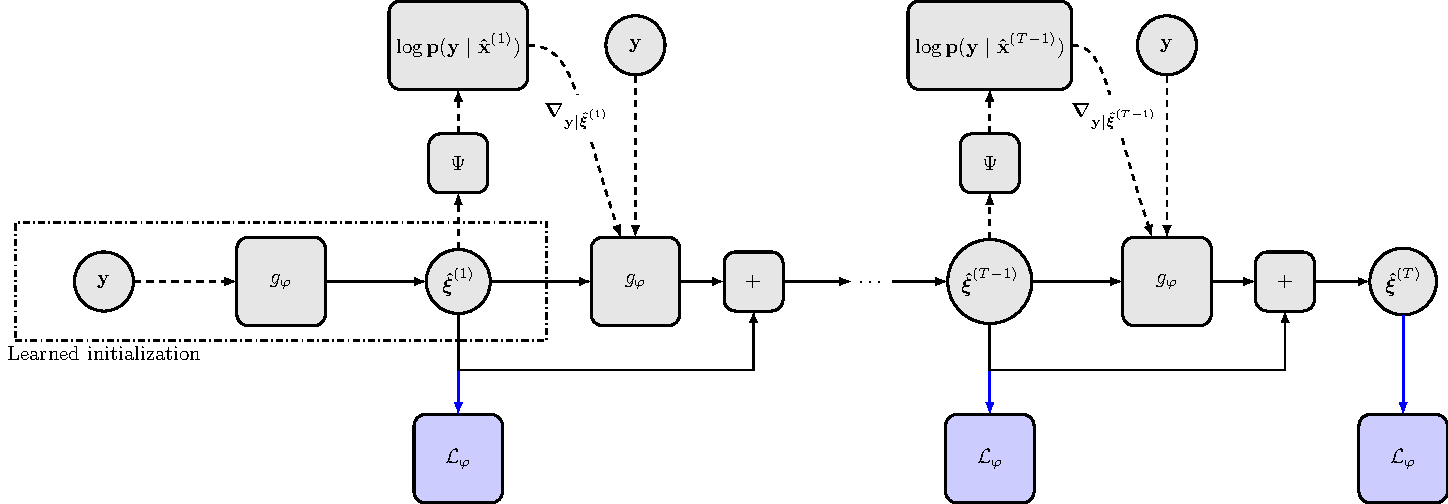
\includegraphics[width=\linewidth]{figures/schematic_rim_unrolled}
        \caption{Unrolled computational graph of the RIM. Operations along solid arrows are being 
        recorded for BPTT, while operations along dashed arrows are not. The blue arrows are only 
        used for optimisation during training. During fine-tuning or testing, the loss is computed only 
        as an oracle metric to validate that our methods can recover the ground truth.}
        \label{fig:unrolled graph}
\end{figure}
\begin{table}[H]
        \centering
        \caption{Hyperparameters for the RIM.}
        \label{tab:baseline hparams}
        \begin{tabular}{cc}
                Parameter & Value \\\hline\hline
                Source link function & $\bbone$ \\
                $\kappa$ link function & $10^{\boldsymbol{\xi}}$ \\
                                       & \\
                \textit{Architecture} & Figure \ref{fig:unet} \\
                Recurrent steps ($T$) & 8 \\
                Number of parameters & $348\,546\,818$ \\
                                      & \\
                \textit{First Stage Optimisation} & \\
                Optimizer & Adamax \\
                Initial learning rate & $10^{-4}$\\
                Learning rate schedule & Exponential Decay \\
                Decay rate & 0.95 \\
                Decay steps & $100\,000$\\
                Number of steps & $610\,000$\\
                Batch size & 1 \\
                           & \\
                \textit{Second Stage Optimisation} & \\
                Optimizer & Adamax \\
                Initial learning rate & $6\times 10^{-5}$\\
                Learning rate schedule & Exponential Decay \\
                Decay rate & 0.9 \\
                Decay steps & $100\,000$\\
                Number of steps & $870\,000$\\
                Batch size & 1 \\
                
                \hline
        \end{tabular}
\end{table}


%\begin{figure}[H]
        %\centering
        %\begin{tikzpicture}
                %\tikzstyle{every node}=[font=\scriptsize]
                %\node at (0, 0) {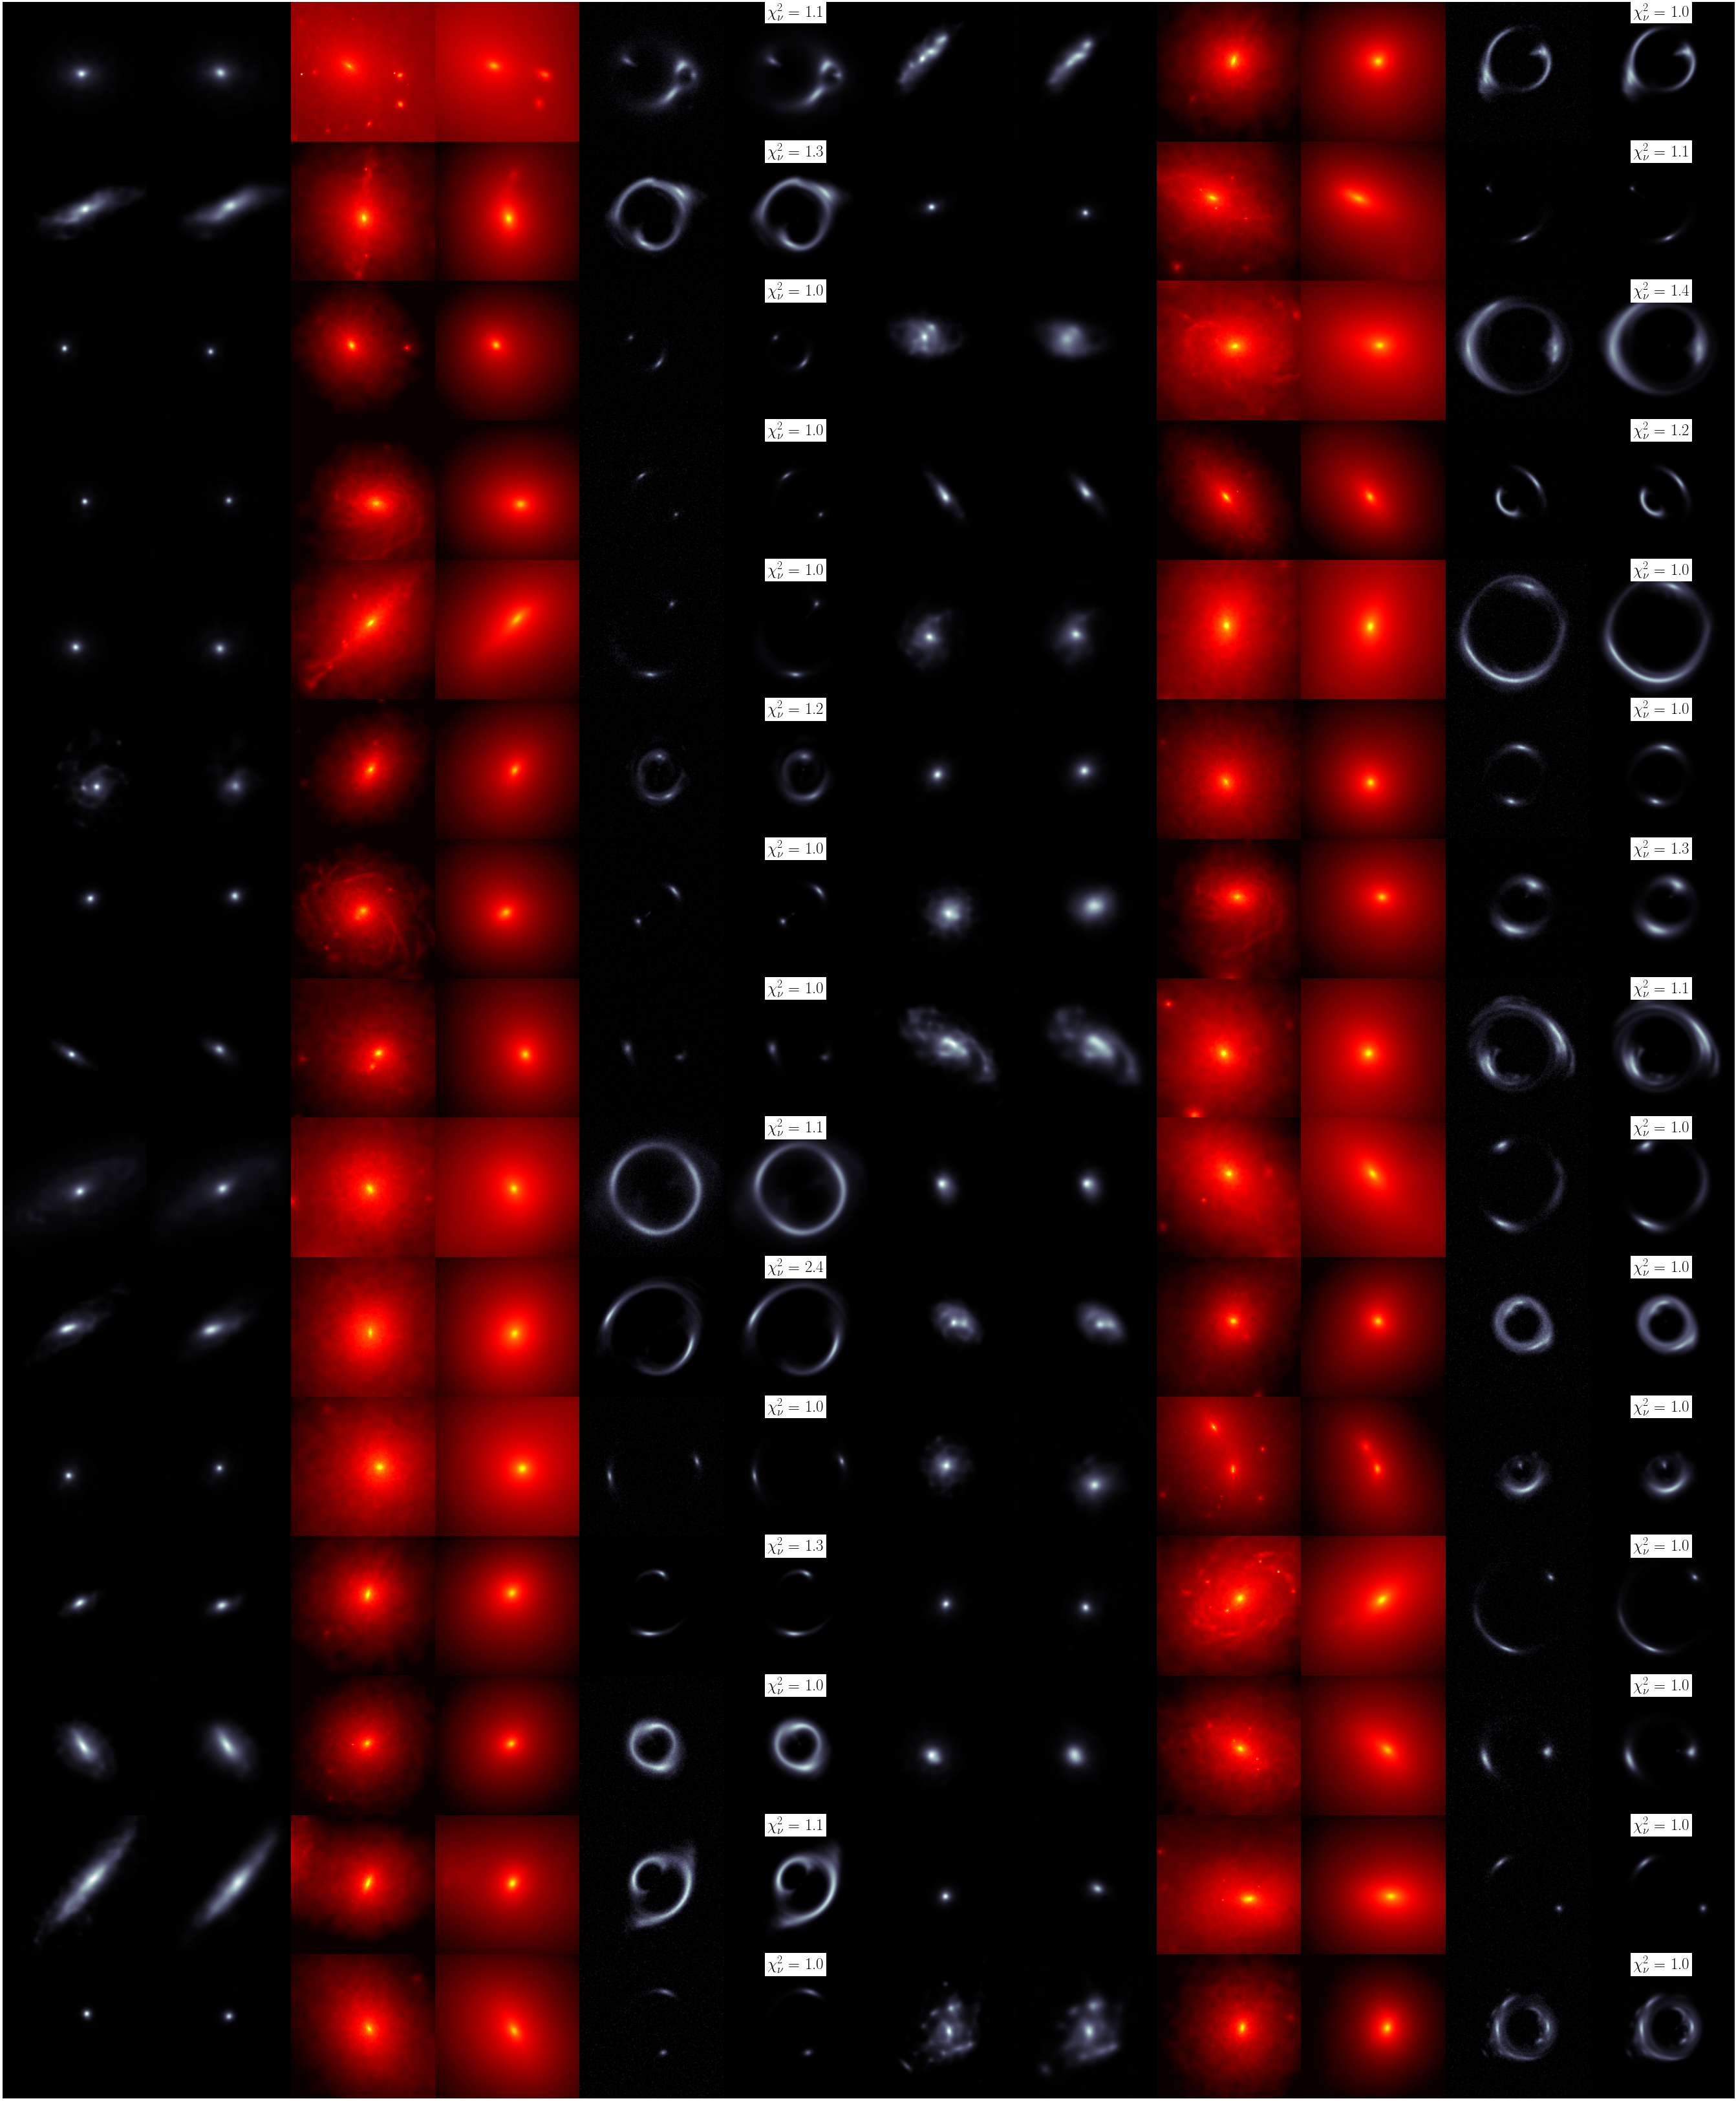
\includegraphics[width=\linewidth]{figures/test_set_no_cherry_pick}};
                %\node at (-8.2, 11) {COSMOS\strut};
                %\node at (-6.8, 11) {RIM+FT\strut};
                %\node at (-5.3, 11) {IllustrisTNG\strut};
                %\node at (-3.7, 11) {RIM+FT\strut};
                %\node at (-2.2, 11) {Observation\strut};
                %\node at (-0.8, 11) {RIM+FT\strut};

                %\node at (0.6, 11) {COSMOS\strut};
                %\node at (2.1, 11) {RIM+FT\strut};
                %\node at (3.7, 11) {IllustrisTNG\strut};
                %\node at (5.2, 11) {RIM+FT\strut};
                %\node at (6.7, 11) {Observation\strut};
                %\node at (8.2, 11) {RIM+FT\strut};

                
                %% \node at (-7.5, 11.2) {COSMOS};
                %% \node at (-4.5, 11.2) {RIM+FT};
                %% \node at (-6, 11.7) {Sources};
                %% \node at (-1.5, 11.2) {Illustris TNG};
                %% \node at (1.5, 11.2) {RIM+FT};
                %% \node at (0, 11.7) {Convergence};
                %% \node at (4.5, 11.2) {Observation};
                %% \node at (7.5, 11.2) {RIM+FT};
        %\end{tikzpicture}
        %\caption{
                %30 reconstructions taken at random from the test set of 3000 examples simulated from COSMOS 
                %and IllustrisTNG data at high SNR.
                %The colorscale are the same as in Figure \ref{fig:main result}.}
        %\label{fig:random sample}
%\end{figure}

